\documentclass[../main.tex]{subfiles}

\begin{document}
\chapter{Differenzierbarkeit}
\section{Differenzierbare Funktionen}
\begin{goal}
  Formalisiere
  folgende Aussage:
  ``der Funktionsgraph einer Funktion
  $f \colon \mathbb{R} \to \mathbb{R}$
  hat im Punkt $(p, f(p))$ eine 
  wohldefinierte Tangente''.
\end{goal}

Affine Funktionen 
\begin{align*}
  A \colon \mathbb{R} & \to \mathbb{R} \\
  x & \mapsto ax + b
\end{align*}
für $a, b \in \mathbb{R}$,
siehe Abbildung~\ref{fig:affin},
sind der Prototyp
einer solchen Funktion.
Für alle $p \in \mathbb{R}$ und
alle $h \in \mathbb{R}$ gilt
\[
  A(p+h) = a(p+ h) + b = A(p) + L(h),
\]
wobei
\begin{align*}
  L \colon \mathbb{R} & \to \mathbb{R} \\
  h & \mapsto ah
\end{align*}
linear ist (im Gegensatz
zu der Funktion
$A \colon \mathbb{R} \to \mathbb{R}$,
welche ``nur'' affin ist).
Wir erhalten, dass für festes $p$ 
gilt, dass
  $A(p+h) = A(p) + L(h)$
die Summe einer konstanten
Funktion mit einer linearen Funktion ist.
Eine solche Aufteilung ist
eine zu restriktive Bedingung
für allgemeinere Funktionen,
da diese nur für affine Funktionen
existiert.


\begin{figure}[htb]
  \centering
  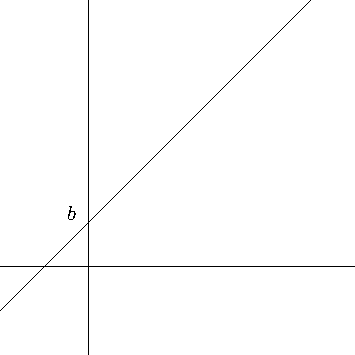
\includegraphics{images/affine}
  \caption{Der
  Graph einer affinen Funktion
$x \mapsto ax + b$}%
  \label{fig:affin}
\end{figure}

\subsection*{Dreigliedentwicklung}
\begin{definition}
  Seien $a, b \in \mathbb{R}$ 
  mit $a < b$ und
  $f \colon (a, b) \to \mathbb{R}$ 
  eine Funktion.
  Weiterhin sei $p \in (a, b)$ und
  $d > 0$ 
  mit $(p - d, p + d) \subset (a, b)$.
  Die Funktion $f \colon (a, b) \to \mathbb{R}$ 
  heisst im Punkt
  $p \in (a, b)$ \emph{differenzierbar},
  falls eine lineare Funktion
  ${(Df)}_p \colon\mathbb{R} \to \mathbb{R}$
  und eine Funktion ${(Rf)}_p \colon (-d, d) \to \mathbb{R}$ 
  existieren, die folgende Eigenschaften erfüllen.
  \begin{enumerate}[(i)]
    \item Für alle $h \in (-d, d)$ gilt
      \[
        f(p + h) = f(p) + {(Df)}_p(h) + {(Rf)}_p(h).
      \]
    \item Für alle $\varepsilon > 0$ existiert
      $\delta > 0$ mit $\delta \leq d$, so dass
      für alle $h \in (- \delta, \delta)$ gilt,
      dass
      \[
        |{(Rf)}_p(h)| \leq \varepsilon \cdot |h|.
      \]
   \end{enumerate}
   Die Aufteilung
   \[
     f(p + h) = f(p) + {(Df)}_p(h) + {(Rf)}_p(h)
   \]
   heisst \emph{Dreigliedentwicklung} von $f$ 
   an der Stelle $p$.
   Die lineare Abbildung
   ${(Df)}_p \colon\mathbb{R} \to \mathbb{R}$ heisst
   \emph{Differential} von $f$ an der Stelle $p$,
   und ${(Rf)}_p$ heisst der \emph{Restterm}.
\end{definition}

Für die Bedingung, dass für
alle $\varepsilon > 0$ ein $\delta > 0$ 
mit $\delta \leq d$ existiert,
so dass für $h \in (-\delta, \delta)$ gilt,
dass
\[
  |{(Rf)}_p(h)| \leq \varepsilon \cdot |h|,
\]
schreiben wir häufig kurz
\[
  \lim_{|h| \to 0} \frac{|{(Rf)}_p(h)|}{|h|} = 0.
\]
Wir sagen auch, dass ${(Rf)}_p \colon (-d, d) \to \mathbb{R}$ \emph{relativ klein}
in $|h|$ ist.

\begin{examples}
  \leavevmode
  \begin{enumerate}[(1)]
    \item Sei $L \colon \mathbb{R} \to \mathbb{R}$ 
      linear.
      Dann gilt für alle $p \in \mathbb{R}$ und alle
      $h \in \mathbb{R}$, dass
      \[
        L(p + h) = L(p) + L(h) + 0.
      \]
      Setze ${(DL)}_p = L \colon \mathbb{R} \to \mathbb{R}$.
      Diese Funktion ist linear. Setze
      ${(RL)}_p(h) = 0$. Diese Funktion erfüllt
      \[
        \lim_{h \to 0} \frac{|{(RL)}_p(h)|}{|h|} = 0.
      \]
      Also ist $L \colon \mathbb{R} \to \mathbb{R}$
      an der Stelle $p \in \mathbb{R}$ 
      differenzierbar mit Differential
      \[
      {(DL)}_p = L \colon \mathbb{R} \to \mathbb{R}.
      \]
    \item Betrachte die Abbildung
      \begin{align*}
        f \colon \mathbb{R} & \to \mathbb{R} \\
        x & \mapsto x^2.
      \end{align*}
      Es gilt für alle $p \in \mathbb{R}$ und
      $h \in \mathbb{R}$, dass
      \[
        f( p + h ) = {(p + h)}^2
        = p^2 + 2ph + h^2
        = f(p) + 2ph + h^2.
      \]
      Setze
      \[
        {(Df)}_p(h) = 2ph
      \]
      und
      \[
        {(Rf)}_p(h) = h^2.
      \]
      Die Funktion
      \begin{align*}
        {(Df)}_p \colon \mathbb{R} & \to \mathbb{R} \\
        h & \mapsto 2ph
      \end{align*}
      ist linear (für festes $p$).
      Die Funktion
      \begin{align*}
        {(Rf)}_p \colon \mathbb{R} & \to \mathbb{R} \\
        h & \mapsto h^2
      \end{align*}
      erfüllt
      \[
        \lim_{h \to 0} \frac{|{(Rf)}_p(h)|}{|h|} = 0.
      \]
      Tatsächlich, sei $\varepsilon > 0$ vorgegeben.
      Setze $\delta = \varepsilon > 0$.
      Für alle $h \in \mathbb{R}$ mit $|h| \leq \delta$ gilt,
      dass
      \[
        |{(Rf)}_p(h)| = |h| \cdot |h| \leq \varepsilon \cdot |h|.
      \]
      Also ist $f$ im Punkt $p \in \mathbb{R}$ differenzierbar
      mit Differential
      \[
        {(Df)}_p(h) = 2p \cdot h.
      \]
  \end{enumerate}
\end{examples}

\subsection*{Eindeutigkeit der Dreigliedentwicklung}
Seien
\[
  f(p + h) = f(p) + {(Df)}_p(h) + {(Rf)}_p(h)
  = f(p) + \widetilde{{(Df)}}_p(h) + \widetilde{{(Rf)}}_p(h)
\]
zwei Dreigliedentwicklungen von $f \colon (a, b) \to \mathbb{R}$.
Dann ist die Funktion
\[
{(Df)}_p - \widetilde{{(Df)}}_p \colon \mathbb{R} \to \mathbb{R}
\]
linear und die Funktion
$
  \widetilde{{(Rf)}}_p- {(Rf)}_p 
$
relativ klein in $|h|$.
Weiter gilt auf dem gemeinsamen Definitionsbereich der
beiden Funktionen, dass
\[
{(Df)}_p - \widetilde{{(Df)}}_p 
  =  \widetilde{{(Rf)}}_p-{(Rf)}_p 
\]


\begin{lemma*}
  Sei $g \colon \mathbb{R} \to \mathbb{R}$ linear und
  relativ klein in $|h|$.
  Dann ist $g$ die Nullfunktion.
\end{lemma*}

\begin{proof}
  Die Funktion $g$ ist linear, das heisst, für alle
  $h \in \mathbb{R}$ gilt
  \[
    g(h) = h \cdot g(1).
  \]
  Weiter ist $g$ relativ klein in $|h|$.
  Sei $\varepsilon > 0$. Dann existiert
  $\delta > 0$ so dass für $|h| \leq \delta$ 
  gilt, dass
  \[
   |g(1)| \cdot |h| = |h \cdot g(1) | = |g(h)| \leq \varepsilon \cdot |h|,
  \]
  also $|g(1)| \leq \varepsilon$.
  Da $\varepsilon > 0$ beliebig war, folgt
  $g(1) = 0$ und somit $g(h) = h \cdot g(1) = 0$.
  In anderen Worten ist $g$ die Nullfunktion.
\end{proof}

\begin{corollary*}
  Die Dreigliedentwicklung ist eindeutig.
\end{corollary*}

\begin{proof}
Seien
\[
  f(p + h) = f(p) + {(Df)}_p(h) + {(Rf)}_p(h)
  = f(p) + \widetilde{{(Df)}}_p(h) + \widetilde{{(Rf)}}_p(h)
\]
zwei Dreigliedentwicklungen von $f \colon (a, b) \to \mathbb{R}$.
Wir haben oben gesehen, dass
\[
  g = 
{(Df)}_p - \widetilde{{(Df)}}_p 
  = \widetilde{{(Rf)}}_p-{(Rf)}_p 
\]
linear und relativ klein in $|h|$, also
die Nullfunktion ist.
\end{proof}

\begin{application}
  Sei $f \colon \mathbb{R} \to \mathbb{R}$ \emph{symmetrisch},
  das heisst, $f(x) = f(-x)$ für alle $x \in \mathbb{R}$,
  und im Punkt $0$ differenzierbar.
  Dann ist ${(Df)}_0 = 0$ die Nullfunktion.

  Tatsächlich, sei
  \[
    f(0 + h) = f(0) + {(Df)}_0(h) + {(Rf)}_0(h)
  \]
  die Dreigliedentwicklung von $f$ bei $p = 0$.
  Da $f$ symmetrisch ist, ist auch
  \[
    f(0 + h) = f(0 - h) = f(0) + {(Df)}_0(-h) + {(Rf)}_0(-h).
  \]
  Mit ${(Df)}_0(-h) = - {(Df)}_0(h)$ und Eindeutigkeit
  der Dreigliedentwicklung folgt, dass
  \[
    {(Df)}_0 = - {(Df)}_0,
  \]
  also ${(Df)}_0(h) = 0$ für alle $h$.
\end{application}


\begin{example}
  Betrachte die Funktion
  \begin{align*}
    f \colon \mathbb{R} & \to \mathbb{R} \\
    x & \mapsto |x|,
  \end{align*}
  siehe Abbildung~\ref{fig:modulus}.
  Dann ist $f$ symmetrisch. Wir behaupten, dass
  $f$ im Punkt $p = 0$ nicht differenzierbar ist.
  Falls doch, muss ${(Df)}_0 = 0$ nach obiger
  Anwendung gelten, also
  folgt
  \[
    |h| = f(0 + h) = f(0) + {(Df)}_0(h) + {(Rf)}_0(h)
    = {(Rf)}_0(h).
  \]
  Aber die Funktion
  \[
    {(Rf)}_0(h) = |h|
  \]
  ist nicht relativ klein in $|h|$. Tatsächlich existiert
  für $\varepsilon < 1$ kein $h \neq 0$ mit
  \[
    |{(Rf)}_p(h)| \leq \varepsilon \cdot |h|.
  \]
  Das ist ein Widerspruch, also ist $f$ im Nullpunkt
  nicht differenzierbar.
\end{example}

\begin{figure}[htb]
  \centering
  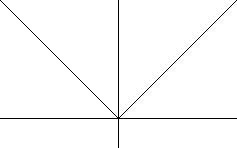
\includegraphics{images/modulus}
  \caption{Der Graph der Funktion $x \mapsto |x|$}%
  \label{fig:modulus}
\end{figure}

\begin{examples}
  \leavevmode
  \begin{enumerate}[(1)]
    \item Sei $f(x) = c$ für eine
      Konstante $c \in \mathbb{R}$.
      Dann gilt für alle $p \in \mathbb{R}$ 
      und $h \in \mathbb{R}$, dass
      \[
        f(p + h) = f(p) + 0 + 0,
      \]
      also ist $f$ differenzierbar und
      ${(Df)}_p = 0$ ist die Nullfunktion.
    \item Sei $f(x) = x^n$ für $n \in \mathbb{N}$
      mit $n \geq 2$. Die Fälle $n = 0$ und $n = 1$ 
      haben wir mit dem konstanten und dem linearen
      Fall bereits behandelt.
      Für alle $p \in \mathbb{R}$ und
      $h \in \mathbb{R}$ gilt
      \[
        f(p + h) = {(p + h)}^n
        = p^n + np^{n-1}h + h^2 \sum_{k=2}^{n} \binom{n}{k}
        p^{n-k}h^{k-2}.
      \]
      Setze nun
      \[
        {(Df)}_p(h) = np^{n-1}h
      \]
      und
      \[
        {(Rf)}_p(h) = h^2 \sum_{k=2}^{n} \binom{n}{k} p^{n-k}h^{k-2}.
      \]
      Dann ist ${(Df)}_p$ linear in $h$.
      Wir behaupten, dass ${(Rf)}_p(h)$ relativ
      klein in $|h|$ ist.
      Sei dazu $\varepsilon > 0$ vorgegeben.
      Setze
      \[
        M = \sum_{k=2}^{n} \binom{n}{k}|p|^{n-k} \geq 0
      \]
      und
      \[
        \delta = \min \{1, \varepsilon / (M + 1)\}.
      \]
      Dann gilt für alle $h \in \mathbb{R}$ 
      mit $|h| \leq \delta$,
      dass
      \[
        |{(Rf)}_p(h)| = |h|^2 \cdot \sum_{k=2}^{n} 
        \binom{n}{k} \cdot |p|^{n-k} \cdot |h|^{k-2}
                 \leq |h|^2 \cdot M % da |h|^{k-2} <= 1
                 \leq |h| \cdot \delta \cdot M 
                 \leq|h| \cdot  \varepsilon.
      \]
      Also ist ${(Rf)}_p(h)$ relativ klein in $|h|$ 
      und somit ist $f$ im Punkt $p$ differenzierbar und
      \[
        {(Df)}_p(h) = n p^{n-1} \cdot h.
      \]
    \item Sei $f(x) = e^x$. Dann ist
      \[
        f(p + h) = e^{p+h} = e^p \cdot e^h
        = e^p \cdot (1  +h + h^2/2! + \cdots)
      \]
      Setze
      \[
        {(Df)}_p(h) = e^p \cdot h
      \]
      und
      \[
        {(Rf)}_p(h) = e^p \cdot (h^2/2! + h^3/3! + \cdots).
      \]
      Dann ist
      \[
        e^{p+h} = e^p + {(Df)}_p(h) + {(Rf)}_p(h)
      \]
      und ${(Df)}_p$ ist linear.
      Dass ${(Rf)}_p(h)$ relativ klein
      in $|h|$ ist, ist eine Aufgabe auf Serie~6.
    \item Sei $f(x) = \log(x)$, definiert auf
      $\mathbb{R}_{>0}$.
      Es ist schwierig, die Dreigliedentwicklung
      von $f$ aufzuschreiben.
    \item Sei $f(x) = \sqrt x$, definiert auf
      $\mathbb{R}_{\geq 0}$.
      Auch für diese Funktion $f$ ist es schwierig,
      die Dreigliedentwicklung aufzuschreiben.
  \end{enumerate}
\end{examples}

Wir werden später sehen, unter welchen Bedingungen
die Umkehrfunktion einer bijektiven
differenzierbaren Funktion differenzierbar ist.

\begin{remarks}
  \leavevmode
  \begin{itemize}
\item
  Für $f(x) = x^n$ und $p \in \mathbb{R}$ beliebig
  gilt
  \[
    {(Df)}_p(h) = n p^{n-1} \cdot h.
  \]
\item
  Für $f(x) = e^x$ und $p \in \mathbb{R}$ beliebig gilt
  \[
    {(Df)}_p(h) = e^p \cdot h.
  \]
  \end{itemize}
  Diese Grössen vor dem $h$ erkennen wir
  wohl wieder.
\end{remarks}

\begin{definition}
  Sei $f \colon (a, b) \to \mathbb{R}$ differenzierbar
  im Punkt $p \in (a, b)$. Dann heisst
  \[
    f'(p) = {(Df)}_p(1)
  \]
  die \emph{Ableitung} von $f$ an der Stelle $p$.
\end{definition}

\begin{proposition*}
  Sei $f \colon (a, b) \to \mathbb{R}$ eine Funktion
  und $p \in (a, b)$ beliebig.
  Dann sind folgende Aussagen äquivalent.
  \begin{enumerate}[\normalfont(i)]
    \item $f$ ist an der Stelle $p$ differenzierbar.
    \item Der Grenzwert
      \[
        \lim_{h \to 0} \frac{f(p+h) - f(p)}{h}
      \]
      existiert.
  \end{enumerate}
  Falls diese Aussagen zutreffen, gilt
  \[
    f'(p) = \lim_{h \to 0} \frac{f(p + h) - f(p)}{h}.
  \]
\end{proposition*}

\begin{remark}
  Wieso verwenden wir nicht den Punkt (ii) der
  Proposition als Definition der Differenzierbarkeit?
  Das hat einen relativ einfachen Grund:
In höheren Dimensionen ist der Ausdruck
$(f(p + h) - f(p))/h$
nicht definiert.
\end{remark}

\begin{example}
  Betrachte die Spiegelung
  \begin{align*}
    f \colon \mathbb{R}^2 & \to \mathbb{R}^2 \\
    (x, y) & \mapsto (x, -y)
  \end{align*}
  an der $x$-Achse, siehe
  Abbildung~\ref{fig:reflection}. Dann ist $f$ linear.

\begin{figure}[htb]
  \centering
  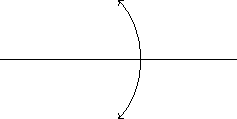
\includegraphics{images/reflection}
  \caption{Spiegelung an der $x$-Achse}%
  \label{fig:reflection}
\end{figure}

  Versuche,
$(f(p + h) - f(p))/h$
auszuwerten. Da $f$ linear ist, folgt
\[
  f(p + h) = f(p) + f(h).
\]
Daraus folgt, 
dass
\[
  \frac{f(p+h) - f(p)}{h} = \frac{f(h)}{h}
  = \frac{(h_1, -h_2)}{(h_1, h_2)}.
\]
Aber das Verhältnis zweier linear unabhängiger
Vektoren ist nicht definiert,
das heisst, der Punkt (ii) in der Proposition
macht keinen Sinn.
Die Funktion $f$ ist aber sehr wohl
nach unserer Definition differenzierbar,
da sie linear ist. Die Dreigliedentwicklung
ist
\[
  f(p + h) = f(p) + f(h) + 0,
\]
also ist ${(Df)}_p = f$.

In der Analysis 2, wenn wir Funktionen
auf höherdimensionalen Räumen
studieren, werden wir also auf
die Dreigliedentwicklung angewiesen sein.
Weiter werden sich alle Beweise, die wir
hier über die Dreigliedentwicklung führen,
auf diese kompliziertere Situation
übertragen lassen.
\end{example}


\begin{proof}[Beweis der Proposition]
  Für die Implikation ``(i) $\Rightarrow$ (ii)''
  sei
  \[
    f(p + h) = f(p) + {(Df)}_p(h) + {(Rf)}_p(h)
  \]
  die Dreigliedentwicklung von $f$ an der
  Stelle $p$.
  Für $h \neq 0$ gilt, dass
  \[
    \frac{f(p + h) - f(p)}{h}
    = \frac{{(Df)}_p(h) + {(Rf)}_p(h)}{h}
    ={(Df)}_p(1) + \frac{{(Rf)}_p(h)}{h}.
  \]
  Da ${(Rf)}_p(h)$ relativ klein in $|h|$ ist,
  folgt dass
  \[
    \lim_{h \to 0} \frac{|{(Rf)}_p(h)|}{|h|} = 0,
  \]
  also auch
  \[
    \lim_{h \to 0} \frac{{(Rf)}_p(h)}{h} = 0.
  \]
  Wir folgern, dass
  \[
    \lim_{h \to 0} \frac{f(p + h) - f(p)}{h}
    = f'(p) + \lim_{h \to 0} \frac{{(Rf)}_p(h)}{h} = f'(p).
  \]
  Insbesondere existiert dieser Grenzwert.

  Wir beweisen nun die Implikation
  ``(ii) $\Rightarrow$ (i)''.
  Nimm an, der Grenzwert
  \[
    a = \lim_{h \to 0} \frac{f(p+h) - f(p)}{h} \in \mathbb{R}
  \]
  existiert.
  Im Hinblick auf $a = f'(p) = {(Df)}_p(1)$
  machen wir den Ansatz
  \[
    f(p + h) = f(p) + a \cdot h + {(Rf)}_p(h)
  \]
  für eine Dreigliedentwicklung von $f$ an der Stelle
  $p \in (a, b)$. Zu zeigen ist, dass
  ${(Rf)}_p(h)$ relativ klein in $|h|$ ist.
  Für $h \neq 0$ gilt
  \[
    \frac{{(Rf)}_p(h)}{h} =
    \frac{f(p+h) - f(p) - ah}{h}
    = \frac{f(p+h) - f(p)}{h} - a.
  \]
  Im Grenzwert gilt also
  \[
    \lim_{h \to 0} \frac{{(Rf)}_p(h)}{h}
    = \lim_{h \to 0}
    \frac{f(p + h) - f(p)}{h} - a
    = a - a = 0.
  \]
  Also folgt auch
  \[
    \lim_{h \to 0} \frac{|{(Rf)}_p(h)|}{|h|} = 0,
  \]
  und somit ist ${(Rf)}_p(h)$ relativ klein
  in $|h|$.
  Wir folgern, dass ${(Df)}_p(h) = a \cdot h$,
  also insbesondere haben wir
  \[
    f'(p) = {(Df)}_p(1) = a = 
    \lim_{h \to 0} \frac{f(p + h) - f(p)}{h}. \qedhere
  \]
\end{proof}

\begin{geometric}
  Die Grösse
  \[
    \frac{f(p+h) - f(p)}{h}
  \]
  ist die Steigung der Sekante
  zwischen den Punkten $(p, f(p))$ 
  und $(p + h, f(p+h))$ im Graphen
  der Funktion $f$, siehe Abbildung~\ref{fig:derivative}
  links.
  Lassen wir $h$ gegen null gehen,
  so erhalten wir im Grenzwert die Tangente
  mit Steigung
  \[
    f'(p) = \lim_{h \to 0} \frac{f(p + h) - f(p)}{h}.
  \]
\end{geometric}

\begin{figure}[htb] 
  \centering
  \begin{minipage}{0.4\textwidth}
    \centering
    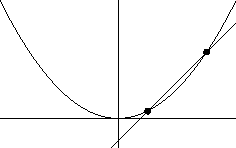
\includegraphics{images/derivative1}
  \end{minipage}%
  \begin{minipage}{0.4\textwidth}
    \centering
    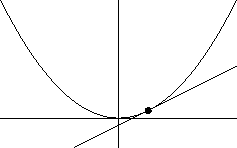
\includegraphics{images/derivative2}
  \end{minipage}%
  \caption{Sekante und Tangente}%
  \label{fig:derivative}
\end{figure}

\begin{examples}
  \leavevmode
  \begin{enumerate}[(1)]
    \item Sei $f(x) = \sqrt x$,
      definiert auf $\mathbb{R}_{\geq 0}$,
      siehe Abbildung~\ref{fig:sqrt}.
      Wir versuchen, die Ableitung
      von $f$ an der Stelle $0$ auszurechnen.
      Berechne
      \[
        \lim_{h \to 0} \frac{f(0 + h) - f(0)}{h}
        = \lim_{h \to 0} \frac{\sqrt h}{h},
      \]
      aber dieser Grenzwert existiert nicht: 
      die Tangente der Funktion im Nullpunkt
      ist vertikal, hat also unendliche Steigung.
      Wir folgern, dass es keine Funktion
      \[
      \overline f \colon (- \delta, \delta) \to \mathbb{R}
      \]
      mit folgenden Eigenschaften gibt.
      \begin{enumerate}[(i)]
        \item $\overline f$ ist differenzierbar
          an der Stelle $p = 0$.
        \item Für alle $x \in [0, \delta]$ gilt
          $\overline f (x) = f(x)$.
      \end{enumerate}
      Allgemeiner würde man Differenzierbarkeit auf
      einem Randpunkt auch über eine solche
      Erweiterung $\overline f$ definieren.
      
      \begin{figure}[htb]
        \centering
        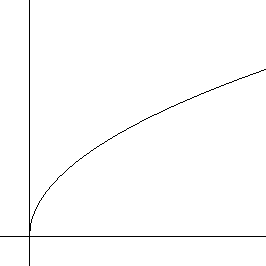
\includegraphics{images/sqrt}
        \caption{Die Wurzelfunktion $f(x) = \sqrt x$}%
        \label{fig:sqrt}
      \end{figure}

    \item Wir definieren die Sinusfunktion geometrisch 
      und untersuchen diese auf Differenzierbarkeit.
      In einem Kreis mit Radius $1$, sei $x$ ein Winkel,
      das heisst, eine Strecke zwischen zwei Punkten auf
      dem Kreis.
      Wir definieren den \emph{Sinus},
      den \emph{Cosinus} und den \emph{Tangens} durch
      \[
        \sin(x) = s \text{, } \cos(x) = c \text{ und }
        \tan(x) = t,
      \]
      wobei $s$, $c$ und $t$ via Abbildung~\ref{fig:sine}
      definiert sind.
      Sowohl der Sinus als auch der Cosinus
      sind also beschränkte Funktionen.
      Es gilt, dass die Verhältnisse
      \[
        c : 1 = s : t
      \]
      übereinstimmen, das heisst
      \[
        t = \frac{s}{c}.
      \]
      Wir bemerken für
      $0 < x < \pi/2$, dass
      \[
        \cos(x) \leq \frac{\sin(x)}{x} \leq 1.
      \]
      Dies folgt aus der geometrischen Tatsache,
      dass $s \leq x \leq t$,
      wovon wir uns vom Bild überzeugen lassen. % x <= t bzw. x >= s kann ich im Bild nicht sehen (Winkel vs. Länge)?
      Also folgt
      \[
        \sin(x) \leq x \leq \frac{\sin(x)}{\cos(x)}.
      \]
      Weiter folgt
      \[
        \lim_{x \to 0} \frac{\sin(x)}{x} = 1,
      \]
      da 
      \[
        \lim_{x \to 0} \cos(x) = 1.
      \]
      Wir folgern, dass
      \[
        \sin'(0) = 
        \lim_{x \to 0} \frac{\sin(x) - \sin(0)}{x}
        = 1.
      \]
      Das heisst, die Funktion 
      $\sin \colon \mathbb{R} \to \mathbb{R}$ ist differenzierbar
      bei $p = 0$.
      Aus den Additionstheoremen folgt leicht,
      dass die Sinusfunktion überall differenzierbar ist.

      \begin{figure}[htb]
        \centering
        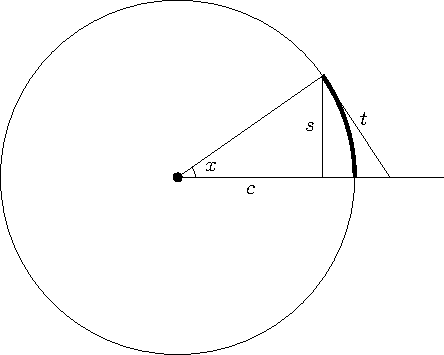
\includegraphics{images/sine}
        \caption{Sinus und Cosinus}%
        \label{fig:sine}
      \end{figure}
    \item Betrachte die Funktion
      \begin{align*}
        f \colon \mathbb{R} & \to \mathbb{R} \\
        x & \mapsto 
        \begin{cases}
          x^2 & \text{falls $x \in \mathbb{Q}$ }, \\
          0 & \text{falls $x \in \mathbb{R} \setminus \mathbb{Q}$ }.
        \end{cases}
      \end{align*}
      Dann ist $f$ an der Stelle $p = 0$ differenzierbar
      und es gilt $f'(0) = 0$. Wir beweisen das mit dem Ansatz
        \[
          f(0 + h) = 0 + 0 + {(Rf)}_0(h)
        \]
      für eine Dreigliedentwicklung bei $p = 0$.
      Zu zeigen ist, dass ${(Rf)}_0(h) = f(h)$ 
      relativ klein in $|h|$ ist.
      Sei dazu $\varepsilon > 0$ vorgegeben.
      Setze $\delta = \varepsilon$.
      Dann gilt für alle $h \in \mathbb{R}$ mit $|h| \leq \delta$,
      dass
      \[
        |{(Rf)}_0(h)| = |f(h)| \leq |h| \cdot |h| \leq \delta \cdot |h|
        = \varepsilon \cdot |h|.
      \]
      In allen Punkten $p \neq 0$ ist $f$ nicht stetig,
      und deshalb auch nicht differenzierbar. Das Letztere
      folgt aus folgendem Lemma.
  \end{enumerate}
\end{examples}

\begin{lemma*}
  Sei $f \colon (a, b) \to \mathbb{R}$ im Punkt $p \in \mathbb{R}$ 
  differenzierbar. Dann ist $f$ im Punkt $p$ stetig.
\end{lemma*}

\begin{proof}[Beweisskizze]
  Das ist eine Übung auf Serie~7.
  Sei $\varepsilon > 0$ vorgegeben. Gesucht
  ist ein $\delta > 0$ so, dass für $h \in \mathbb{R}$ 
  mit $|h| \leq \delta$ gilt, dass
  $|f(p+h) - f(p)| \leq \varepsilon$.
  Nach der Dreigliedentwicklung ist aber
  \[
    |f(p + h) - f(p)| = |{(Df)}_p(h) - {(Rf)}_p(h)|
    \leq |h \cdot f'(p)| + |{(Rf)}_p(h)|
  \]
  Wähle nun $\delta > 0$ geeignet.
\end{proof}

\begin{remark}
  Es existieren stetige Funktionen $f \colon \mathbb{R} \to \mathbb{R}$,
  welche in keinem Punkt differenzierbar sind.
  Solche Funktionen wurden erstmals vom deutschen Mathematiker
  Weierstrass konstruiert.
\end{remark}

\section{Die Kettenregel}

\begin{chainrule}
Seien 
$a, b, c, d \in \mathbb{R}$ mit $a < b$ und $c < d$,
sei $g \colon (a, b) \to \mathbb{R}$ 
eine Funktion,
deren Bild in $(c, d)$ liegt, das heisst,
$g((a, b)) \subset (c, d)$,
und sei $f \colon (c, d) \to \mathbb{R}$ eine Funktion.
Falls $g$ im Punkt $p \in (a, b)$ und $f$ 
im Punkt $g(p) \in (c, d)$ differenzierbar sind,
dann ist die Komposition
$f \circ g \colon (a, b) \to \mathbb{R}$ 
im Punkt $p$ differenzierbar, und es gilt
\[
  {(D(f \circ g))}_p = {(Df)}_{g(p)} \circ {(Dg)}_p.
\]
\end{chainrule}

\begin{remark}
  Da $g'(p) = {(Dg)}_p(1)$ und
  ebenso $f'(g(p)) = {(Df)}_{g(p)}(1)$,
  haben wir, dass
  \begin{align*}
    (f \circ g)'(p)
    & = {(D(f \circ g))}_p(1) \\
    & = {(Df)}_{g(p)} \circ {(Dg)}_p(1) \\
    & = {(Df)}_{g(p)}(g'(p)) \\
    & = g'(p) \cdot {(Df)}_{g(p)}(1) \\
    & = g'(p) \cdot f'(g(p)),
  \end{align*}
  oder in einer Zeile,
  \[
    (f \circ g)'(p) = f'(g(p)) \cdot g'(p),
  \]
  was auch häufig als die \emph{Kettenregel}
  bezeichnet wird.
\end{remark}

\begin{proof}[Beweis der Kettenregel]
  Wir leiten eine Dreigliedentwicklung
  für $f \circ g$ an der Stelle $p \in (a, b)$ her.
  Schreibe mithilfe der Dreigliedentwicklung
  von $g$, dass
  \begin{align*}
    f \circ g(p + h) 
    &= f(g(p+h))  \\
    &= f(g(p) + {(Dg)}_p(h) + {(Rg)}_p(h)) \\
    &= f(g(p) + \overline h)
  \end{align*}
  für $\overline h = {(Dg)}_p(h) + {(Rg)}_p(h)$.
  Wir können nun die Dreigliedentwicklung von $f$ 
  anwenden um zu sehen, dass
  \[
    f \circ g(p + h) = f(g(p)) + {(Df)}_{g(p)}(\overline h)
    + {(Rf)}_{g(p)}(\overline h).
  \]
  Nach Linearität von ${(Df)}_{g(p)}$ gilt, dass
  \[
    f(g(p+h)) = f(g(p)) + {(Df)}_{g(p)}(
    {(Dg)}_p(h))
    + {(Df)}_{g(p)}({(Rg)}_p(h))
    + {(Rf)}_{g(p)}(\overline h).
  \]
  Setze
  \[
    {(D(f \circ g))}_p(h) = {(Df)}_{g(p)}({(Dg)}_p(h)).
  \]
  Setzen wir
  \[
    R_1(h) = {(Df)}_{g(p)}({(Rg)}_p(h))
  \]
  und
  \[
    R_2(h) = {(Rf)}_{g(p)}(\overline h),
  \]
  so bleibt zu zeigen, dass $R_1(h)$ 
  und $R_2(h)$ relativ klein
  in $|h|$ sind.
  \begin{enumerate}[(1)]
    \item Berechne
      \begin{align*}
        R_1(h)
        & = {(Rg)}_p(h) \cdot {(Df)}_{g(p)}(1)\\
        & = {(Rg)}_p(h) \cdot f'(g(p)),
      \end{align*}
      wobei $f'(g(p))$ konstant ist.
      Das heisst, $R_1(h)$ ist das
      Produkt einer Konstanten mit
      einem Term, der relativ klein in $|h|$ ist.
      Also ist $R_1(h)$ relativ klein in $|h|$.
    \item Berechne
      \[
        R_2(h) 
        = {(Rf)}_{g(p)}({(Dg)}_p(h) + {(Rg)}_p(h)).
      \]
      Sei $\varepsilon > 0$ vorgegeben. Wähle
      $\delta_1 > 0$ so, dass
      für $h \in \mathbb{R}$ mit $|h| \leq \delta_1$ gilt,
      dass
      \[
        |{(Rg)}_p(h)| \leq |h|.
      \]
      Dann ist also
      \begin{align*}
         |\overline h| 
         & = |{(Dg)}_p(h) + {(Rg)}_p(h)|\\
         & \leq |{(Dg)}_p(h)| + |{(Rg)}_p(h)| \\
         &\leq |g'(p)| \cdot |h| + |h| \\
         &= (|g'(p)| + 1) \cdot |h| \\
         &= \alpha \cdot |h|
      \end{align*}
      für $\alpha = |g'(p)| + 1$.
      Wähle nun $\delta_2 > 0$ so,
      dass für alle $\widetilde h \in \mathbb{R}$ 
      mit $|\widetilde h| \leq \delta_2$ gilt,
      dass
      \[
        |{(Rf)}_{g(p)}(\widetilde h)| \leq \varepsilon/\alpha
        \cdot |\widetilde h|.
      \]
      Dann gilt für alle $h \in \mathbb{R}$ mit
      $|h| \leq \delta_1$ und $|h| \leq \delta_2/\alpha$,
      dass
      \[
        |R_2(h)| = |{(Rf)}_{g(p)}(\overline h)|
        \leq \varepsilon/\alpha \cdot |\overline h| \leq
        \varepsilon \cdot |h|.
      \]
      Hier haben wir verwendet, dass
      $|\overline h| \leq \alpha \cdot |h| \leq \delta_2$,
      was wir aus $|h| \leq \delta_1$ schliessen
      können. \qedhere
  \end{enumerate}
\end{proof}

\subsection*{Anwendungen der Kettenregel}
\subsubsection*{Ableitungen von Umkehrfunktionen}
Sei $f \colon (a, b) \to (c, d)$ 
differenzierbar und bijektiv.
Dann existiert eine Umkehrfunktion
von $f$, das heisst, eine Funktion
$g \colon (c, d) \to (a, b)$ 
mit $f \circ g = \text{Id}_{(c, d)}$,
die Identität des Intervalls
$(c, d)$. Das heisst, für alle
$x \in (c, d)$ gilt
\[
  f(g(x)) = x.
\]
Falls $g$ im Punkt $p \in (c, d)$
differenzierbar ist, dann gilt
\[
  {(D(\text{Id}_{(c, d)}))}_{p} = 
  {(D(f \circ g))}_p
  = {(Df)}_{g(p)} \circ {(Dg)}_p.
\]
Da das Differential einer linearen Abbildung
die lineare Abbildung selbst ist,
folgt insbesondere, dass
\[
  {(D(\text{Id}_{(c, d)}))}_p = \text{Id}_{\mathbb{R}}.
\]
Wir folgern, dass
\[
  {(Df)}_{g(p)} \circ {(Dg)}_p = \text{Id}_{\mathbb{R}},
\]
das heisst, die beiden linearen Abbildungen
${(Df)}_{g(p)} \colon \mathbb{R} \to \mathbb{R}$
und ${(Dg)}_p \colon \mathbb{R} \to \mathbb{R}$ 
sind zueinander invers.
Für die Ableitungen gilt, dass
\[
  f'(g(p)) \cdot g'(p) = 1,
\]
also
\[
  g'(p) = \frac{1}{f'(g(p))}.
\]

\begin{example}
Betrachte
\begin{align*}
  f \colon \mathbb{R} & \to \mathbb{R}_{>0} \\
  x & \mapsto e^x.
\end{align*}
Wir wissen bereits, dass $f'(x) = e^x$ gilt.
Die Umkehrfunktion
\begin{align*}
  g \colon \mathbb{R}_{>0} & \to \mathbb{R} \\
  x & \mapsto \log(x)
\end{align*}
erfüllt also, falls $g$ im Punkt $p > 0$ differenzierbar ist,
\[
  g'(p) = \frac{1}{f'(g(p))} = \frac{1}{p}.
\]
Falls $\log \colon \mathbb{R}_{>0} \to \mathbb{R}$ 
differenzierbar ist, dann gilt somit
\[
  \log'(x) = \frac{1}{x}.
\]
\end{example}
      
\begin{warning}
  Aus $f(g(x)) = x$ und $f$ differenzierbar
  folgt nicht, dass $g$ differenzierbar ist.
\end{warning}

\begin{example}
  Betrachte
  \begin{align*}
    f \colon \mathbb{R} & \to \mathbb{R} \\
    x & \mapsto x^3.
  \end{align*}
  Die Umkehrfunktion von $f$ ist
  \begin{align*}
    g \colon \mathbb{R} & \to \mathbb{R} \\
    x & \mapsto \sqrt[3]{x},
  \end{align*}
  welche aufgrund einer vertikalen Tangente im
  Nullpunkt, siehe Abbildung~\ref{fig:cube},
  nicht differenzierbar ist.
  
\end{example}

\begin{figure}[htb] 
  \centering
  \begin{minipage}{0.40\textwidth}
    \centering
    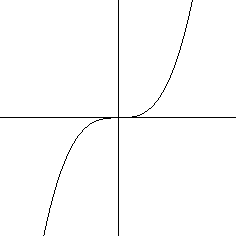
\includegraphics{images/cube-1}
  \end{minipage}%
  \begin{minipage}{0.40\textwidth}
    \centering
    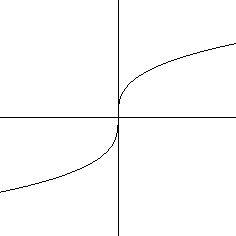
\includegraphics{images/cube-2}
  \end{minipage}%
  \caption{Die Umkehrfunktion von $x \mapsto x^3$
  ist im Nullpunkt nicht differenzierbar.}%
  \label{fig:cube}
\end{figure}

\subsubsection*{Die Quotientenregel}
Betrachte die Funktion
\begin{align*}
  f \colon \mathbb{R} \setminus \{0\} & \to \mathbb{R} \\
  x & \mapsto \frac{1}{x}.
\end{align*}
Dann gilt für 
$p \neq 0$ und für $h \in \mathbb{R}$ mit $p + h \neq 0$, dass
\[
  \frac{f(p+h) - f(p)}{h} = \frac{\frac{1}{p+h} - \frac{1}{p}}{h}
  = \frac{-1}{p(p+h)},
\]
also
\[
  \lim_{h \to 0} \frac{f(p+h) - f(p)}{h} = - \frac{1}{p^2}.
\]
Somit ist $f$ an der Stelle
$p \neq 0$ differenzierbar und es gilt
\[
  f'(p) = \frac{-1}{p^2}.
\]
Sei nun $g \colon \mathbb{R} \to \mathbb{R} \setminus \{0\}$ 
differenzierbar an der Stelle $p \in \mathbb{R}$.
Dann gilt
\[
  (f \circ g)'(p) = f'(g(p)) \cdot g'(p)
  = -\frac{g'(p)}{{g(p)}^2}.
\]
Zusammengefasst erhalten wir die \emph{Quotientenregel}
\[
  \left( \frac{1}{g(x)} \right)' = -\frac{g'(x)}{{g(x)}^2}
\]

\subsection*{Die Produktregel}
\begin{productrule}
Seien $f, g \colon (a, b) \to \mathbb{R}$ 
im Punkt $p \in (a, b)$ differenzierbar.
Dann ist das Produkt
$f \cdot g \colon (a, b) \to \mathbb{R}$ 
im Punkt $p$ differenzierbar und es gilt
\[
  {(D(f \cdot g))}_p(h) = f(p) \cdot
  {(Dg)}_p(h) + g(p) \cdot {(Df)}_p(h)
\]
\end{productrule}

\begin{remark}
  Für die Ableitung gilt
  \[
    {(f\cdot g)}'(p) = f(p) \cdot g'(p) + g(p) \cdot f'(p),
  \]
  was auch häufig als die \emph{Produktregel}
  bezeichnet wird.
  Dies folgt direkt via einsetzen von $h = 1$.
\end{remark}

\begin{proof}[Beweisskizze]
  Wir leiten eine Dreigliedentwicklung für $f \cdot g$ 
  bei $p$ wie folgt her. Berechne
  \begin{align*}
    (f \cdot g) (p+h)
    & = f(p+h) \cdot g(p+h)\\
    &= \left( f(p) + {(Df)}_p(h) + {(Rf)}_p(h) \right)
    \cdot \left( g(p) + {(Dg)}_p(h) + {(Rg)}_p(h) \right) \\
    &= (f \cdot g)(p)
    + f(p) \cdot {(Dg)}_p(h) + g(p) \cdot {(Df)}_p(h)
    + {(R(f \cdot g))}_p(h),
  \end{align*}
  wobei ${(R(f \cdot g))}_p$ aus $6$ Resttermen
  besteht.
  Bemerke, dass
  \[
    {(D(f \cdot g))}_p(h) = f(p) \cdot {(Dg)}_p(h)
    + g(p) \cdot {(Df)}_p(h)
  \]
  linear in $h$ ist.
  Die $6$ Restterme sind
  \begin{itemize}
    \item $f(p) \cdot {(Rg)}_p(h)$ und
      $g(p) \cdot {(Rf)}_p(h)$, welche beide
      ein Produkt einer Konstanten
      mit einem Term, der relativ klein in $|h|$ ist, sind, % oder m.E. besser: "; beide sind Produkte einer Konstanten mit einem Term, der relativ klein in $|h|$;"
    \item ${(Df)}_p(h) \cdot {(Rg)}_p(h)$,
      ${(Rf)}_p(h) \cdot {(Dg)}_p(h)$ und
      ${(Rf)}_p(h) \cdot {(Rg)}_p(h)$,
      welche nicht allzu schwierig zu untersuchen sind,
    \item ${(Df)}_p(h) \cdot {(Dg)}_p(h) = h^2
      \cdot f'(p) \cdot g'(p)$, was ein Produkt
      einer Konstanten
      mit $h^2$ und somit relativ klein in $|h|$ ist.
  \end{itemize}
  Da die Summe von relativ kleinen Termen selbst relativ
  klein ist, haben wir die Produktregel bewiesen.
\end{proof}

\section{Der Mittelwertsatz}
\begin{question}
  Sei $f \colon \mathbb{R} \to \mathbb{R}$ 
  differenzierbar mit $f' = 0$ (die Nullfunktion),
  das heisst, für alle $x \in \mathbb{R}$ gilt
  $f'(x) = 0$. Ist dann $f$ konstant?
\end{question}

Die Antwort ist (ausnahmsweise) ja.
Das ist aber nicht ganz trivial, da wir
die Integralrechnung noch nicht aufgebaut haben.
Wir brauchen dafür den Mittelwertsatz
(nicht zu verwechseln mit dem Zwischenwertsatz).

\begin{meanvalue}
  Sei $f \colon [a, b] \to \mathbb{R}$ 
  stetig und differenzierbar auf $(a, b)$.
  Dann existiert $p \in (a, b)$ mit $f(b) - f(a)
  = f'(p) \cdot (b-a)$.
\end{meanvalue}

\begin{geometric}
  Sei $ f \colon [a, b] \to \mathbb{R}$ stetig
  und differenzierbar auf $(a, b)$.
  Dann existiert $p \in (a, b)$ so, dass
  die Sehne zwischen $(a, f(a))$ und
  $(b, f(b))$ dieselbe Steigung
  wie die Tangente des Graphen von $f$ zu $
  (p, f(p))$ hat. Siehe Abbildung~\ref{fig:meanvalue}.
\end{geometric}

\begin{figure}[htb]
  \centering
  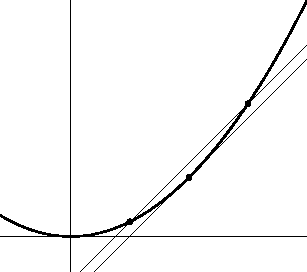
\includegraphics{images/meanvalue}
  \caption{Geometrische Interpretation
  des Mittelwertsatzes}%
  \label{fig:meanvalue}
\end{figure}

Ein Spezialfall des Mittelwertsatzes ist folgender Satz.

\begin{rolle}
  Sei $h \colon [0, 1] \to \mathbb{R}$ stetig
  und differenzierbar auf $(0, 1)$ 
  mit $h(0) = h(1)$.
  Dann existiert $t \in (0, 1)$ 
  mit $h'(t) = 0$.
\end{rolle}

\begin{figure}[htb]
  \centering
  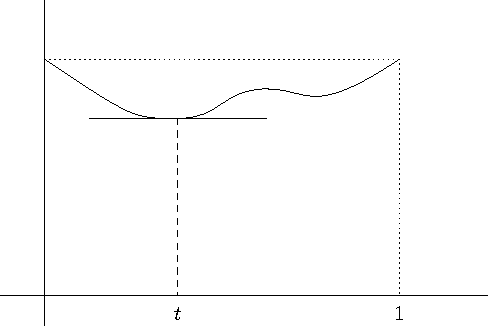
\includegraphics{images/rolle}
  \caption{Satz von Rolle}%
  \label{fig:rolle}
\end{figure}

\begin{proof}
  Wir unterscheiden drei Fälle.
  \begin{enumerate}[1.]
    \item $h$ ist konstant.
      Dann gilt für alle $t\in (0, 1)$,
      dass $h'(t) = 0$.
    \item Es existiert $p \in (0, 1)$ 
      mit $h(p) < h(0) = h(1)$.
      Das ist die Situation, die in
      Abbildung~\ref{fig:rolle} dargestellt ist.
      Da $h \colon [0, 1] \to \mathbb{R}$ 
      stetig ist, nimmt $h$ auf dem
      kompakten Intervall
      $[0, 1]$ ein Minimum an.
      Es existiert also $t \in [0, 1]$
      so, dass für alle $q \in [0, 1]$ 
      gilt, dass
      $h(t) \leq h(q)$.
      Wegen $h(p) < h(0) = h(1)$ folgt,
      dass $t \in (0, 1)$.
      Wir behaupten nun, dass $h'(t) = 0$.
      Für den Beweis, siehe das Lemma unten.
    \item Es existiert $p \in (0, 1)$ mit
      $h(p) > h(0) = h(1)$. Wie im 2. Fall
      folgt die Existenz eines Maximums
      an einer Stelle $t \in (0, 1)$.
      Auch hier folgt aus dem Lemma unten,
      dass $h'(t) = 0$. \qedhere
  \end{enumerate}
\end{proof}

\begin{definition}
  Sei $h \colon (a, b) \to \mathbb{R}$ differenzierbar.
  Wir sagen, dass $h$ an der Stelle
  $p \in (a, b)$ ein \emph{lokales
  Minimum} annimmt, falls $\delta > 0$
  mit $ (p - \delta, p + \delta)
  \subset (a, b)$ existiert,
  so dass für alle $q \in (p - \delta, p + \delta)$
  gilt, dass  $h(q) \geq h(p)$. Ähnlich sagen wir,
  dass $h$ an der Stelle
  $p \in (a, b)$ ein \emph{lokales Maximum}
  annimmt, falls $\delta > 0$ mit
  $(p - \delta, p + \delta) \subset (a, b)$
  existiert, so dass für alle $q \in (p - \delta, p + \delta)$ 
  gilt, dass $h(q) \leq h(p)$.
  Wir sagen weiterhin, dass $h$ an der
  Stelle $p \in (a, b)$ ein
  \emph{lokales Extremum} annimmt, falls 
  $h$ an der Stelle $p$
  ein lokales Maximum oder ein lokales Minimum
  annimmt.
\end{definition}


\begin{lemma*}
  Sei $h \colon (a, b) \to \mathbb{R}$
  differenzierbar mit einem lokalen
  Extremum an einer Stelle
  $p \in (a, b)$. Dann gilt $h'(p) = 0$.
\end{lemma*}

\begin{remark}
  Die Umkehrung gilt nicht: Nur weil $h'(t) = 0$ 
  gilt, heisst das nicht, dass~$t$ ein
  lokales Extremum von $h$ ist.
\end{remark}

\begin{example}
  Betrachte die Funktion
  \begin{align*}
    h \colon \mathbb{R} & \to \mathbb{R} \\
    x & \mapsto x^3,
  \end{align*}
  siehe Abbildung~\ref{fig:cube} links.
  Dann gilt $h'(0) = 0$, aber $h$
  hat kein lokales Extremum im Nullpunkt.
\end{example}

\begin{proof}[Beweis des Lemmas]
  Wir nehmen an, dass $h$ an der Stelle
  $p$ ein lokales Minimum annimmt. Der Fall,
  dass $h$ ein lokales Maximum bei $p$ annimmt,
  ist analog.
  Sei
  \begin{align*}
    h(p+k)
    & = h(p) + {(Dh)}_p(k) + {(Rh)}_p(k)\\
    & = h(p) + h'(p) \cdot k + {(Rh)}_p(k).
  \end{align*}
  Wir unterscheiden nun drei Fälle,
  wobei zwei davon zu einem Widerspruch führen werden.
  \begin{enumerate}[(1)]
    \item $h'(p) = 0$. Das wollen wir zeigen.
    \item $h'(p) > 0$. Setze
      \[
        \varepsilon = \frac{h'(p)}{2} > 0.
      \]
      Dann existiert $\delta > 0$ so dass
      für alle $k \in \mathbb{R}$ mit
      $|k| \leq \delta$ gilt, dass
      $|{(Rh)}_p(k)| \leq \varepsilon \cdot |k|$.
      Für alle $k \in (0, \delta)$ gilt:
      \begin{align*}
        h(p-k)
        &= h(p) - k \cdot h'(p) + {(Rh)}_p(-k)\\
        &\leq h(p) - k \cdot h'(p) + \frac{h'(p)}{2} \cdot k \\
        &= h(p) - \frac{h'(p)}{2} \cdot k \\
        &< h(p),
      \end{align*}
      was der Annahme, dass $h$ ein lokales Minimum bei $p$
      hat, widerspricht.
    \item $h'(p) < 0$.
      Setze 
      \[
        \varepsilon = \frac{|h'(p)|}{2} > 0.
      \]
      Dann existiert wie im 2. Fall $\delta > 0$ so dass
      für alle $k \in \mathbb{R}$ mit
      $|k| \leq \delta$ gilt, dass
      $|{(Rh)}_p(k)| \leq \varepsilon \cdot |k|$.
      Für alle $k \in (0, \delta)$ gilt dann
      analog
      $h(p + k) < h(p)$, was auch ein Widerspruch ist. \qedhere
  \end{enumerate}
\end{proof}

\begin{proof}[Beweis des Mittelwertsatzes]
  Betrachte die Hilfsfunktion 
  \begin{align*}
    h \colon [0, 1] & \to \mathbb{R} \\
    t & \mapsto f((1- t)a + tb) - (1-t) \cdot f(a) - t\cdot f(b).
  \end{align*}
  Für $t \in (0, 1)$ gilt
  \[
    (1- t) \cdot a + t \cdot b = a + t \cdot (b-a) \in (a, b).
  \]
  Die Funktion $h$ ist stetig auf dem Intervall $[0, 1]$,
  da sie eine Verknüpfung stetiger Funktionen ist,
  und differenzierbar auf $(0, 1)$, da sie eine Verknüpfung
  differenzierbarer Funktionen ist.
  Es gilt
  \begin{align*}
    h(0) &= f(a) - f(a) = 0,\\
    h(1) & = f(b) - f(b) = 0.
  \end{align*}
  Nach dem Satz von Rolle folgt, dass
  $t_0 \in (0, 1)$ mit $h'(t_0) = 0$ 
  existiert.
  Wir berechnen \[
    h'(t)  = f'((1-t)a + tb) \cdot (b-a) 
  + f(a) - f(b). \]
  Setze nun
  \[
    p = (1- t_0) \cdot a + t_0 \cdot b \in (a, b).
  \]
  Es gilt
  \[
    0 = h'(t_0) = f'(p) \cdot (b-a) + f(a) - f(b),
  \]
  also
  \[
    f'(p) = \frac{f(b) - f(a)}{b-a}. \qedhere
  \]
\end{proof}

\begin{corollary}
  Sei $f \colon \mathbb{R} \to \mathbb{R}$ differenzierbar
  mit $f' = 0$, die Nullfunktion.
  Dann ist $f$ konstant.
\end{corollary}

\begin{proof}
  Sei $a < b$. Nach dem Mittelwertsatz
  existiert $p \in (a, b)$ mit
  \[
    f(b) - f(a) = f'(p) \cdot (b-a) = 0,
  \]
  also $f(b) = f(a)$.
  Dies gilt für alle $a < b$, also
  ist $f$ konstant.
\end{proof}

\begin{definition}
  Eine Funktion $f \colon (a, b) \to \mathbb{R}$ 
  heisst \emph{stetig differenzierbar}, falls
  $f$ differenzierbar und $f' \colon (a, b) \to \mathbb{R}$ 
  stetig ist.
\end{definition}


\begin{corollary}\label{cor:strictly-monotone}
  Sei $f \colon (a, b) \to \mathbb{R}$ 
  stetig differenzierbar und sei
  $p \in (a, b)$ mit $f'(p) > 0$.
  Dann existiert $\delta > 0$,
  so dass $f|_{(p- \delta, p + \delta)}
  \colon (p - \delta, p + \delta) \to \mathbb{R}$ 
  streng monoton wachsend ist,
  das heisst, für alle $x, y \in (p - \delta, p + \delta)$ 
  mit $x < y$ gilt
  $f(x) < f(y)$.
\end{corollary}

\begin{proof}
  Setze
  \[
    \varepsilon = \frac{f'(p)}{2} > 0.
  \]
  Da $f'$ stetig im Punkt $p$ ist, existiert
  $\delta > 0$ so, dass
  \begin{enumerate}[(i)]
    \item $(p - \delta, p + \delta) \subset (a, b)$,
    \item für alle $q \in (p - \delta, p + \delta)$ 
      gilt
      \[
        |f'(q) - f'(p)| \leq \varepsilon.
      \]
  \end{enumerate}
  Insbesondere gilt dann für
  $q \in (p - \delta, p + \delta)$, dass
  \[
    f'(q) \geq f'(p) - \varepsilon \geq \frac{f'(p)}{2} > 0.
  \]
  Seien nun $x, y \in (p - \delta, p + \delta)$ mit
  $x < y$.
  Nach dem Mittelwertsatz existiert $t \in (x, y)$
  mit 
  \[f(y)  - f(x) = f'(t) \cdot (y - x) > 0. \]
  Also gilt $f(y) > f(x)$.
\end{proof}

\subsection*{Konvexität}
Mithilfe des Mittelwertsatzes können wir Folgendes zeigen.
\begin{enumerate}[(i)]
  \item 
    Sei $f \colon \mathbb{R} \to \mathbb{R}$ differenzierbar
    mit $f' \geq 0$, das heisst, für alle $x \in \mathbb{R}$ 
    gilt $f'(x) \geq 0$.
    Dann ist $f$ monoton wachsend.
    Tatsächlich, seien $x, y \in \mathbb{R}$ mit $x < y$.
    Dann existiert $p \in (x, y)$ mit
    \[
      0 \leq f'(p) \cdot (y - x) = f(y) - f(x),
    \]
    also gilt $f(x) \leq f(y)$.
  \item
    Sei $f \colon \mathbb{R} \to \mathbb{R}$ zweimal
    differenzierbar, das heisst, $f$ ist differenzierbar
    und $f'$ ist differenzierbar mit $f'' \geq 0$.
    Dann ist $f'$ monoton wachsend.
    Wende dazu Punkt (i) auf
    $f' \colon\mathbb{R} \to \mathbb{R}$ 
    an.
    Salopp gesagt heisst das,
    dass die Steigung der Tangenten an den
    Funktionsgraph von $f$ von links nach rechts
    zunimmt.
\end{enumerate}

\begin{definition}
  Eine Funktion $f \colon \mathbb{R} \to \mathbb{R}$ 
  heisst \emph{konvex}, falls für alle $a, b, c \in \mathbb{R}$ 
  mit $a < c < b$ der Punkt
  $(c, f(c))
  \in \mathbb{R}^2$ unter
  oder auf der Gerade durch die Punkte
  $(a, f(a))$ und $(b, f(b))$ liegt,
  siehe Abbildung~\ref{fig:convexity}.
\end{definition}

\begin{figure}[htb]
  \centering
  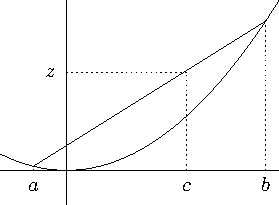
\includegraphics{images/convexity}
  \caption{Konvexität}%
  \label{fig:convexity}
\end{figure}

Formaler, schreibe
$
  c = a + t \cdot (b-a)
  $
mit $t \in (0, 1)$.
Berechne den Schnittpunkt $(c, z)$ der
Geraden $g$ zwischen
$(a, f(a))$ und $(b, f(b))$ 
mit der vertikalen Geraden durch $(c, 0)$ 
folgendermassen:
\[
  z = f(a) + t \cdot (f(b) - f(a)).
\]
Die \emph{Konvexitätsbedingung} ist also
$f(c) \leq z$, das heisst,
\[
  f(a + t \cdot (b-a)) \leq f(a) + t\cdot (f(b) - f(a)).
\]
Wir können also die Definition oben folgendermassen
umformulieren.

\begin{definition}
  Eine Funktion $f \colon \mathbb{R} \to \mathbb{R}$ 
  heisst \emph{konvex}, falls für alle $a < b$ 
  und $t \in [0, 1]$ gilt, dass
  \[
    f(a + t \cdot (b - a)) \leq f(a) + t\cdot (f(b) - f(a)).
  \]
\end{definition}

\newpage
\begin{remarks}
  \leavevmode
  \begin{enumerate}[(1)]
    \item Falls $f \colon \mathbb{R} \to \mathbb{R}$ 
      zweimal differenzierbar ist und $f'' \geq 0$ gilt,
      so ist $f$ konvex. Siehe dazu Serie 8.
    \item Nicht jede konvexe Funktion
      $f \colon \mathbb{R} \to \mathbb{R}$ ist
      differenzierbar.
  \end{enumerate}
\end{remarks}

\begin{example}
  Betrachte die Funktion
  \begin{align*}
    f \colon \mathbb{R} & \to \mathbb{R} \\
    x & \mapsto |x|,
  \end{align*}
  siehe Abbildung~\ref{fig:modulus}.
  Diese Funktion $f$ ist konvex, aber im
  Nullpunkt nicht differenzierbar.
  Aber $f$ ist stetig.
\end{example}

\begin{claim}
  Jede konvexe Funktion $f \colon \mathbb{R} \to \mathbb{R}$ 
  ist stetig.
\end{claim}

\begin{proof}[Beweisskizze]
  Sei $x \in \mathbb{R}$.
  Betrachte die Geraden $g$ 
  durch $(x, f(x))$ und $(x-1, f(x-1))$
  und $h$ durch $(x, f(x))$ und $(x+  1, f(x+1))$.
  Dann liegt der Funktionsgraph von $f$ 
  über dem Intervall $[x-1, x+1]$ zwischen
  $g$ und $h$, siehe Abbildung~\ref{fig:convex-continuous}.
  Das liegt daran, dass bei der Postulation
  eines beliebigen Punktes ausserhalb
  der grauen Region eine Sehne auftaucht,
  die über dem Funktionsgraph von $f$ liegt.
  Es folgt, dass
  \[
    \lim_{q \to x} f(q) = f(x),
  \]
  das heisst, $f$ ist stetig in $x$.
\end{proof}

\begin{figure}[htb]
  \centering
  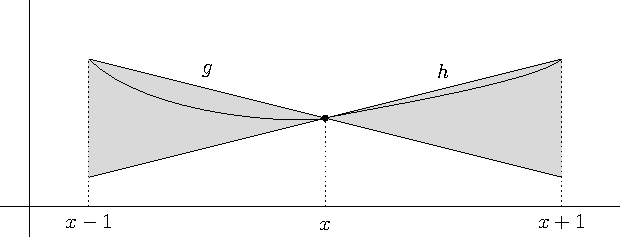
\includegraphics{images/convex-continuous}
  \caption{Konvexe Funktionen sind stetig}%
  \label{fig:convex-continuous}
\end{figure}

Mit einer Variation vom obigen Argument lässt sich zeigen,
dass konvexe Funktionen differenzierbar in allen
bis auf abzählbar vielen Punkten sind.

\section{Der Umkehrsatz}
\begin{question}
  Sei $f \colon (a, b) \to \mathbb{R}$ differenzierbar
  und $p \in (a, b)$ mit $f'(p) > 0$.
  Existiert $\delta > 0$, so dass
  $f|_{(p - \delta, p + \delta)} \colon
  (p - \delta, p + \delta)$ streng monoton wachsend ist?
\end{question}

In Korollar~\ref{cor:strictly-monotone} haben wir das
nicht bewiesen, da wir dort stetige
Differenzierbarkeit gefordert haben.
Tatsächlich ist die Antwort nein.

\begin{example}
  Betrachte zunächst die Funktion
  \begin{align*}
    g \colon \mathbb{R} & \to \mathbb{R} \\
    x & \mapsto
    \begin{cases}
      0, & \text{falls $x = 0$}, \\
      x^2 \cdot \sin(1/x), & \text{sonst}.
    \end{cases}
  \end{align*}
Es gilt
\[
  g'(0) = \lim_{h \to 0} \frac{g(h) - g(0)}{h}
  = \lim_{h \to 0} h \cdot \sin(1/h) = 0,
\]
da $|\sin(1/h)| \leq 1$ gilt.
Für $x \neq 0$ gilt
\[
  g'(x) = 2x \cdot \sin(1/x) + x^2 \cdot \cos(1/x) \cdot (-1/x^2)
  = 2x \cdot \sin(1/x) - \cos (1/x).
\]
Insbesondere gilt für alle $n \in \mathbb{Z}$ mit
$n \neq 0$, dass
\[
  g'(1/2\pi n) = -1.
\]
Betrachte nun
\begin{align*}
  f \colon \mathbb{R} & \to \mathbb{R} \\
  x & \mapsto x + 2g(x).
\end{align*}
Dann ist $f$ differenzierbar und es gilt
\[
  f'(0) = 1 + g'(0) = 1
\]
und
\[
  f'(1/2 \pi n) = 1 + 2 \cdot g'(1/ 2 \pi n) = -1
\]
für alle $n \in \mathbb{Z}$ mit $n \neq 0$.
Insbesondere existiert keine offene
Umgebung von $p = 0$,
in welcher $f$ monoton wachsend ist,
obwohl $f'(0) = 1$.
Das Problem hier ist, dass
$f'$ an der Stelle $p = 0$ nicht stetig ist.
\end{example}

\begin{inverse}
  Sei $f \colon (a, b) \to \mathbb{R}$ stetig
  differenzierbar und $p \in (a, b)$ mit $f'(p) > 0$.
  Dann existiert $\delta > 0$ so, dass
  die Einschränkung $f|_{(p - \delta, p + \delta)}
  \colon (p - \delta, p + \delta) \to
  (f(p - \delta), f(p + \delta))$
  bijektiv und die Umkehrfunktion
  $g = f|_{(p - \delta, p + \delta)}^{-1}$ 
  differenzierbar ist und fűr alle
  $q \in (f(p-\delta), f(p + \delta))$ die Bedingung
  \[
    g'(q) = \frac{1}{f'(g(q))}
  \]
  erfüllt.
\end{inverse}

\begin{remark}
  Es ist wichtig, dass
  $f$ stetig differenzierbar ist.
  Die Funktion $f(x) = x + 2 x^2 \sin(1/x)$ 
  erfüllt $f'(0) = 1$, aber  $f$ ist in
  keiner offenen Umgebung von $0$ 
  umkehrbar, siehe obiges Beispiel.
\end{remark}

\begin{proof}
  Wähle $\delta > 0$ so, dass
  \begin{enumerate}[(i)]
    \item $[p - \delta, p + \delta] \subset (a,b)$,
    \item fűr alle $q \in (p - \delta, p + \delta)$ gilt
      \[
        |f'(q) - f'(p)| \leq \frac{f'(p)}{2}.
      \]
  \end{enumerate}
  Insbesondere gilt für alle $q \in (p - \delta, p + \delta)$, dass
  \[
    f'(q) \geq \frac{f'(q)}{2} > 0.
  \]
  Nach dem Mittelwertsatz ist $f$ auf dem
  Intervall $(p -\delta, p+\delta)$ streng
  monoton wachsend, also injektiv.
  Nach dem Zwischenwertsatz für stetige Funktionen
  nimmt $f$ auf dem Intervall $(p - \delta, p + \delta)$ 
  jeden Wert zwischen $f(p - \delta)$ und $f(p + \delta)$ an.
  Daraus folgt, dass die Einschränkung
  $f|_{(p - \delta, p + \delta)} \colon (p - \delta, p + \delta) \to (c, d)$,
  wobei
  $c = f(p - \delta)$ und $d = f(p + \delta)$,
  bijektiv ist.

  Sei $g = f|_{(p - \delta, p + \delta)}^{-1}$ die
  Umkehrfunktion.
  Zu zeigen ist, dass $g$ differenzierbar ist.
  Sei dazu $q \in (c, d)$ und $h \in \mathbb{R}$ so dass
  $q + h \in (c, d)$. 
  Setze $\tilde q = g(q) \in (p - \delta, p +\delta)$ und
  $\tilde h = g(q + h) - g(q)$.
  Mit dieser Wahl gilt, dass
  \[
    f(\tilde q) = f(g(q)) = q
  \]
  und
  \[
    f(\tilde q + \tilde h) = f(g(q + h)) = q + h.
  \]
  Nach dem Mittelwertsatz existiert $t \in (\tilde q, \tilde q + \tilde h)$ 
  mit
  \[
    h = f(\tilde q + \tilde h) - f(\tilde q) = f'(t) \cdot \tilde h.
  \]
  Berechne nun
  \[
    \frac{g(q + h) - g(q)}{h} = \frac{\tilde h}{h} =
    \frac{\tilde h}{f(\tilde q + \tilde h) - f(\tilde q) } =
    \frac{1}{f'(t)}.
  \]
  Bemerke, dass für $t \in (\tilde q, \tilde q + \tilde h) \subset (p - \delta, p + \delta)$ 
  gilt, dass
  $f'(t) \geq f'(p) / 2 > 0$, also ist $1/f'(t)$ definiert.
  Im Grenzűbergang $h \to 0$ erhalten wir
  \[
    \lim_{h \to 0} \tilde h = \lim_{h \to 0} \frac{h}{f'(t)} = 0,
  \]
  da $f'(t) \geq f'(p) / 2$, und somit folgt
  \[
    \lim_{h \to 0} t = \tilde q,
  \]
  da $t \in (\tilde q, \tilde q + \tilde h)$. Wir folgern,
  dass
  \[
    \lim_{h \to 0} \frac{g(q + h) - g(q)}{h} = \frac{1}{f'(\tilde q)} = \frac{1}{f'(g(q))}.
  \]
  Also ist $g$ im Punkt $q \in (f(p - \delta), f(p + \delta))$ differenzierbar
  und es gilt wie gefordert $g'(q) = 1 / f'(g(q))$.
\end{proof}

\begin{examples}
  \leavevmode
  \begin{enumerate}[(1)]
    \item Betrachte $f = \exp \colon \mathbb{R} \to \mathbb{R}_{>0}$.
      Wir bemerken, dass $f$ stetig differenzierbar ist, da $f' = f$.
      Weiterhin gilt für alle $x \in \mathbb{R}$, dass
      $f'(x) = e^x > 0$, also ist die Umkehrfunktion $g = \log$ 
      auf $\mathbb{R}_{>0}$ differenzierbar mit
      \[
        g'(x) = \frac{1}{f'(g(x))} = \frac{1}{f(g(x))} = \frac{1}{x}.
      \]
      Für $x > 0$ gilt also
       \[
         \log'(x) = 1 / x.
      \]
    \item Betrachte die Funktion
      \begin{align*}
        f \colon \mathbb{R}_{> 0} & \to \mathbb{R}_{> 0} \\
        x & \mapsto x^2.
      \end{align*}
      Dann gilt $g(x) = \sqrt x$. Bemerke, dass
      $f'(x) = 2x$ stetig ist.
      Weiterhin gilt für alle $x > 0$, dass $f'(x) = 2 x > 0$.
      Also ist $g$ im Punkt $x^2$ differenzierbar,
      also auf ganz $\mathbb{R}_{>0}$. Für alle
      $x > 0$ gilt
      \[
        g'(x) = \frac{1}{f'(g(x))} = \frac{1}{2 \sqrt x}.
      \]
      Zusammengefasst erhalten wir
      \[
        \sqrt x ' = \frac{1}{2\sqrt x}.
      \]      
  \end{enumerate}
\end{examples}

\subsection*{Winkelfunktionen}
Wir erinnern uns an die geometrische Überlegung, dass
die Sinusfunktion
$\sin$ 
an der Stelle $x = 0$ differenzierbar ist mit
$\sin'(0) = 1$. Weiter gilt nach dem Satz
von Pythagoras für alle $x \in \mathbb{R}$,
dass
\[
  {(\cos(x))}^2 + {(\sin(x))}^2 = 1,
\]
also 
\[
  \cos(x) = \sqrt{1 - \sin^2(x)}.
\]
Gemäss Beispiel (2) und der
Kettenregel ist $\cos$ an der
Stelle $x = 0$ differenzierbar
und es gilt
\[
  \cos ' ( 0 ) = 
  \frac{1}{2 \sqrt{1 - \sin(0)}} \cdot (-2 \cdot \sin(0) \cdot \sin'(0)) = 0.
\]

\begin{question}
  Sind $\sin$ und $\cos$ auch an Stellen $x \neq 0$
  differenzierbar?
\end{question}

Die Antwort ist ja. Verwende dazu das Additionstheorem
\[
  \sin(x + y) = \sin(x) \cdot \cos(y) + \cos(x) \cdot \sin(y)
\]
um zu zeigen, dass
\begin{align*}
  \frac{\sin( x + h ) - \sin(x)}{h}
  &=
  \frac{\sin(x) \cdot \cos(h) + \cos(x) \cdot \sin(h) - \sin(x)}{h}
  \\ & 
  = \sin(x) \cdot \frac{\cos(h) - \cos(0)}{h} + \cos(x) \cdot \frac{\sin(h) - \sin(0)}{h}.
\end{align*}
Es folgt, dass
\[
  \sin'(x) = \lim_{h \to 0} \frac{\sin(x + h) - \sin(x)}{h} =
  \sin(x) \cdot \cos'(0) + \cos(x) \cdot \sin' (0),
\]
also
\[
  \sin'(x) = \cos x
\]
und ebenso
\[
  \cos'(x) = -\sin(x).
\]
Um das Additionstheorem, das wir verwendet haben, zu beweisen,
betrachte die Drehungen $D_x, D_y, D_{x + y}$ um den Nullpunkt
in $\mathbb{R}^2$ mit Winkeln $x, y, x + y $.
Es gilt $D_{x + y} = D_x \circ D_y$, also folgt
\[
  \begin{pmatrix}
    \cos( x + y ) & - \sin(x + y) \\
    \sin( x + y ) & \cos(x + y)
  \end{pmatrix}
  =
  \begin{pmatrix}
    \cos(x) & -\sin(x) \\
    \sin(x) & \cos(x)
  \end{pmatrix}
  \cdot
  \begin{pmatrix}
    \cos(y) & -\sin(y) \\
    \sin(y) & \cos(y)
  \end{pmatrix}.
\]
Die gesuchte Formel steht dann in einer Komponente
der resultierenden Matrizen.


\end{document}
